\chapter{Evolution of the STXS framework}\label{app:merging_schemes}

\section{Stage 0}
\begin{figure}[htb!]
  \centering
  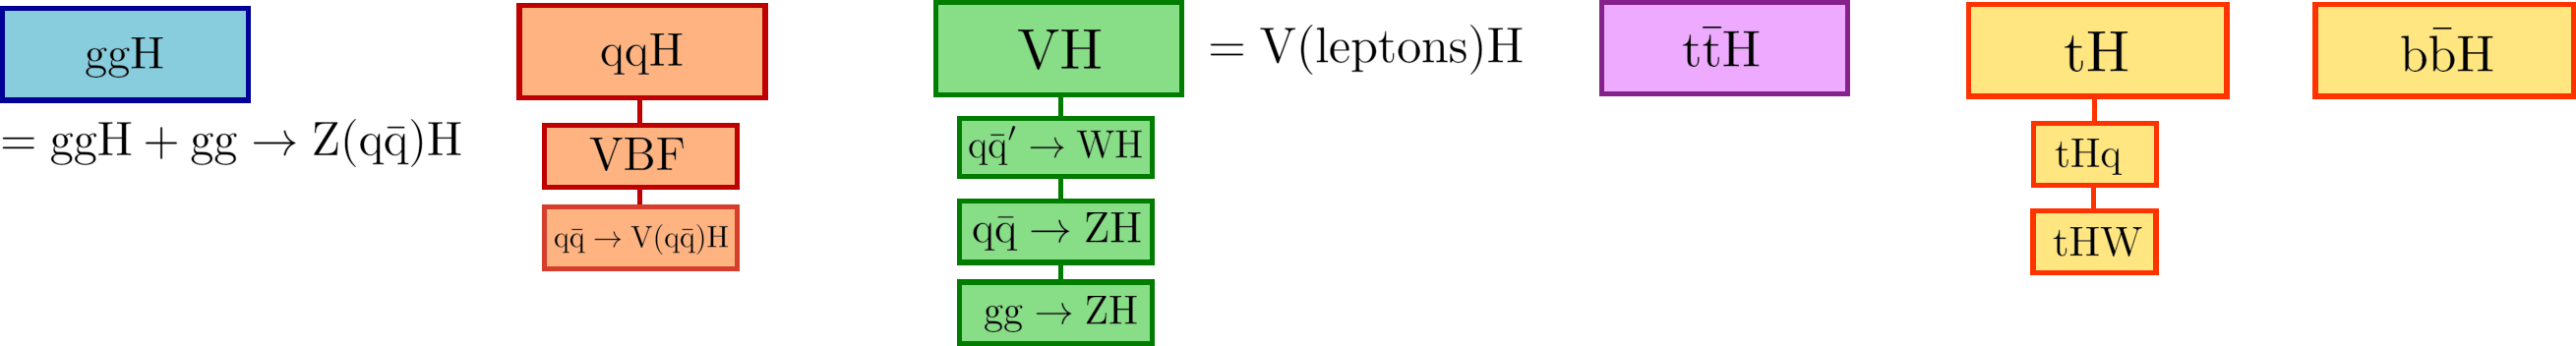
\includegraphics[width=1\linewidth]{Figures/app_merging_schemes/stage0.pdf}
  \caption[Schematic of the STXS stage 0 binning scheme]
  {
    Add caption
  }
  \label{fig:stxs_schematic_stage0}
\end{figure}

\FloatBarrier
\section{Stage 1.0}
\begin{figure}[htb!]
  \centering
  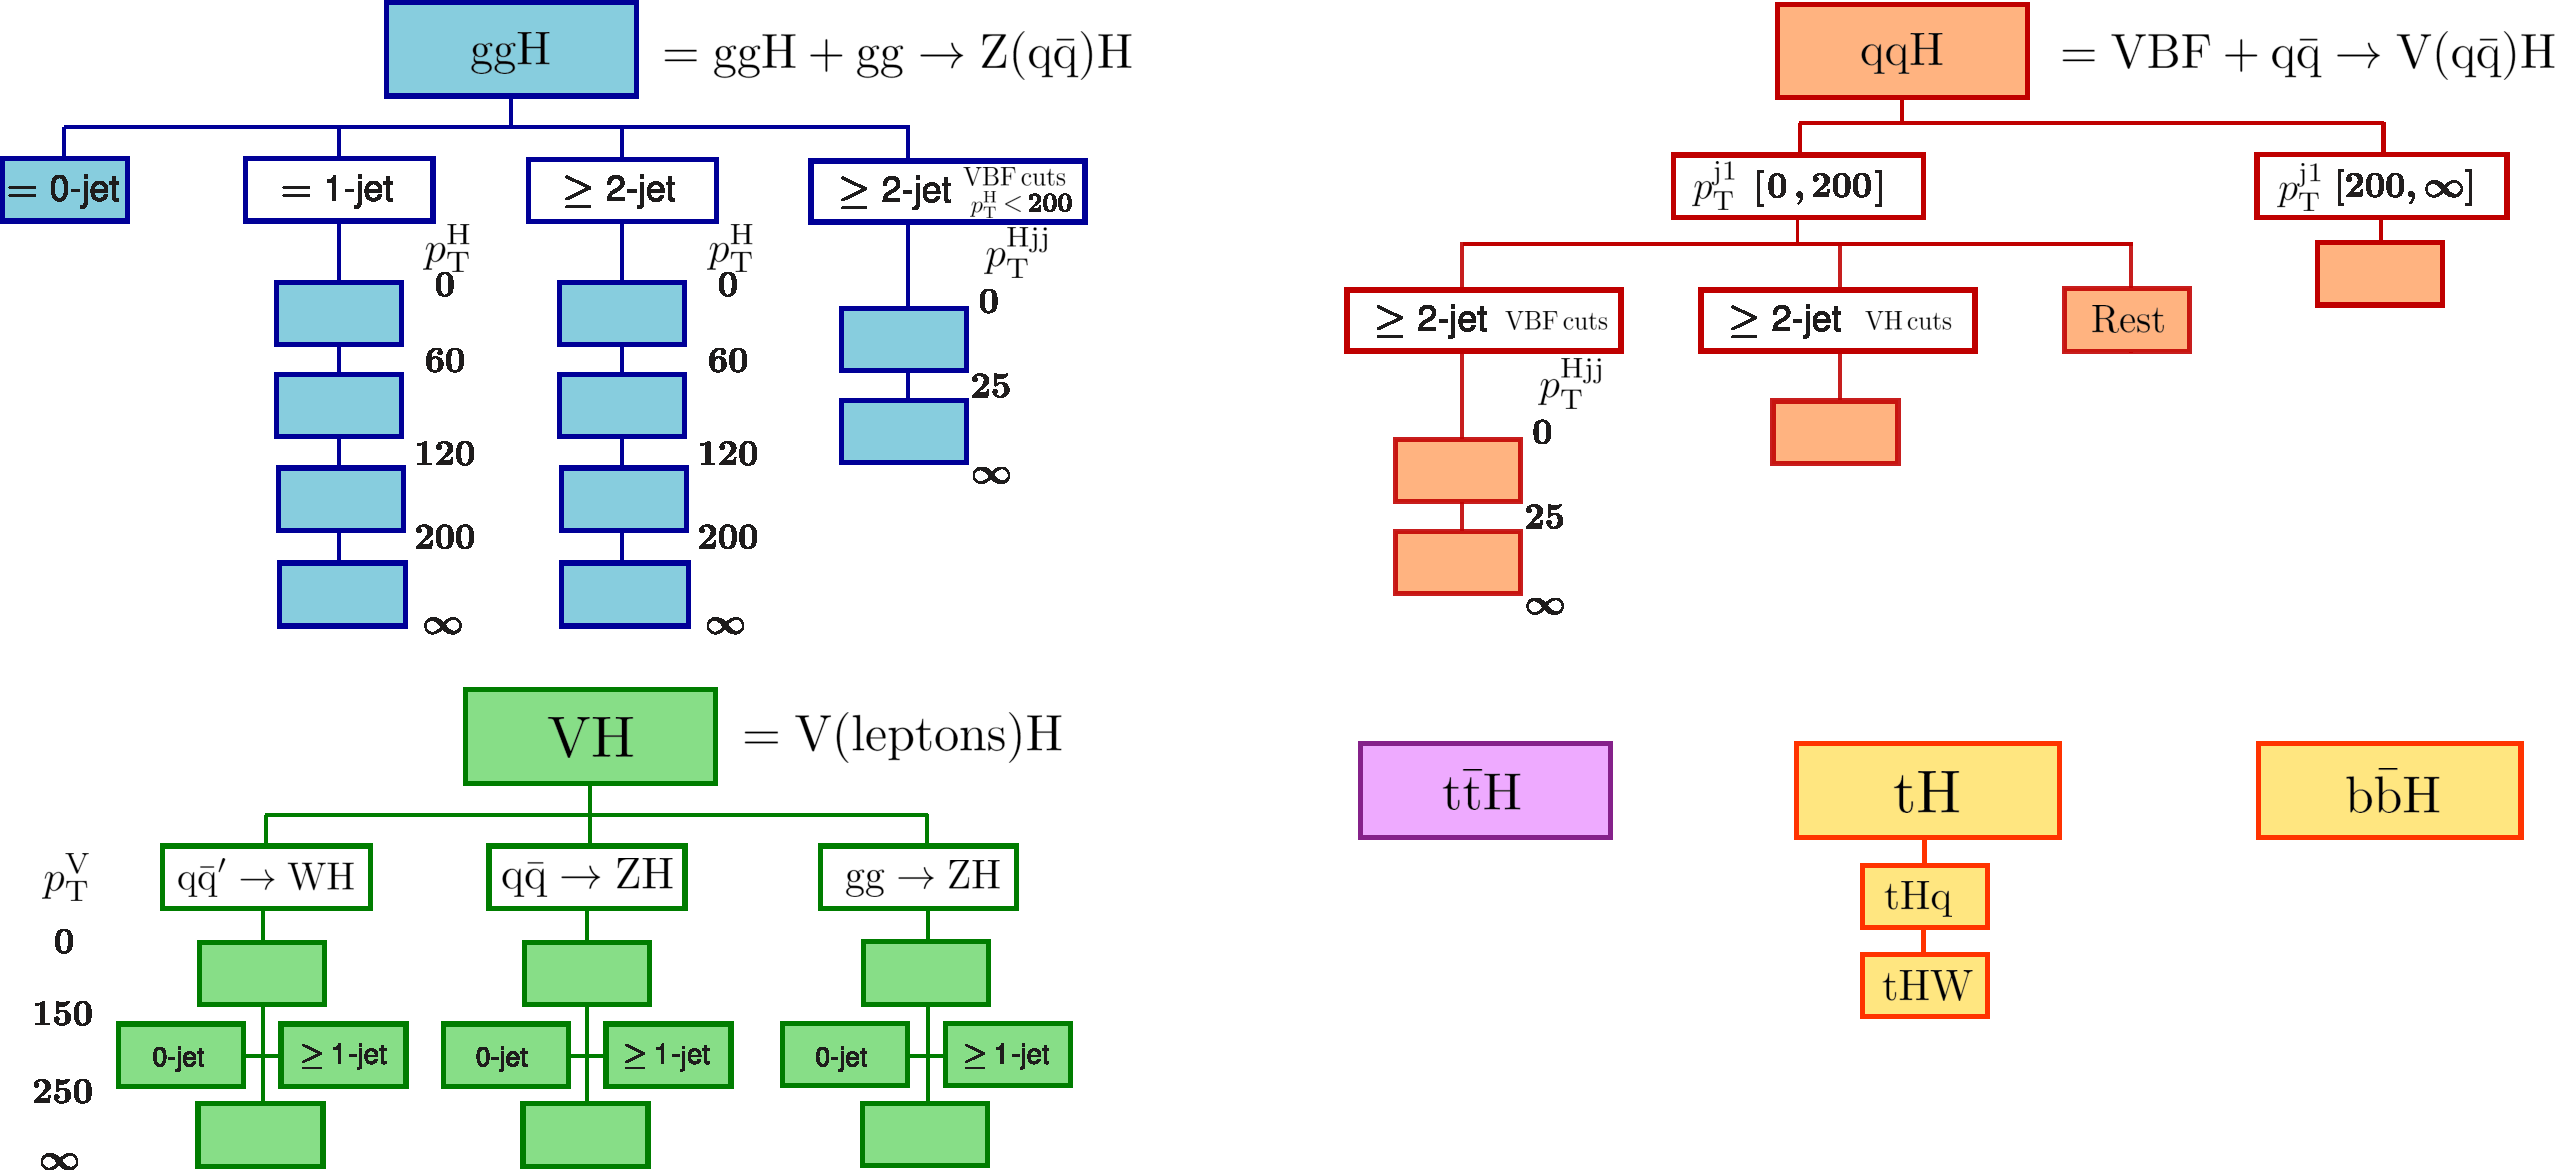
\includegraphics[width=1\linewidth]{Figures/app_merging_schemes/stage1p0.pdf}
  \caption[Schematic of the STXS stage 1.0 binning scheme]
  {
    Add caption. Define what is meant by VBF and VH cuts: $m_{jj}>400$ and $\Delta\eta_{jj}>2.8$, $60<m_{jj}<120$
  }
  \label{fig:stxs_schematic_stage1p0}
\end{figure}

\FloatBarrier
\section{Stage 1.1}
\begin{figure}[htb!]
  \centering
  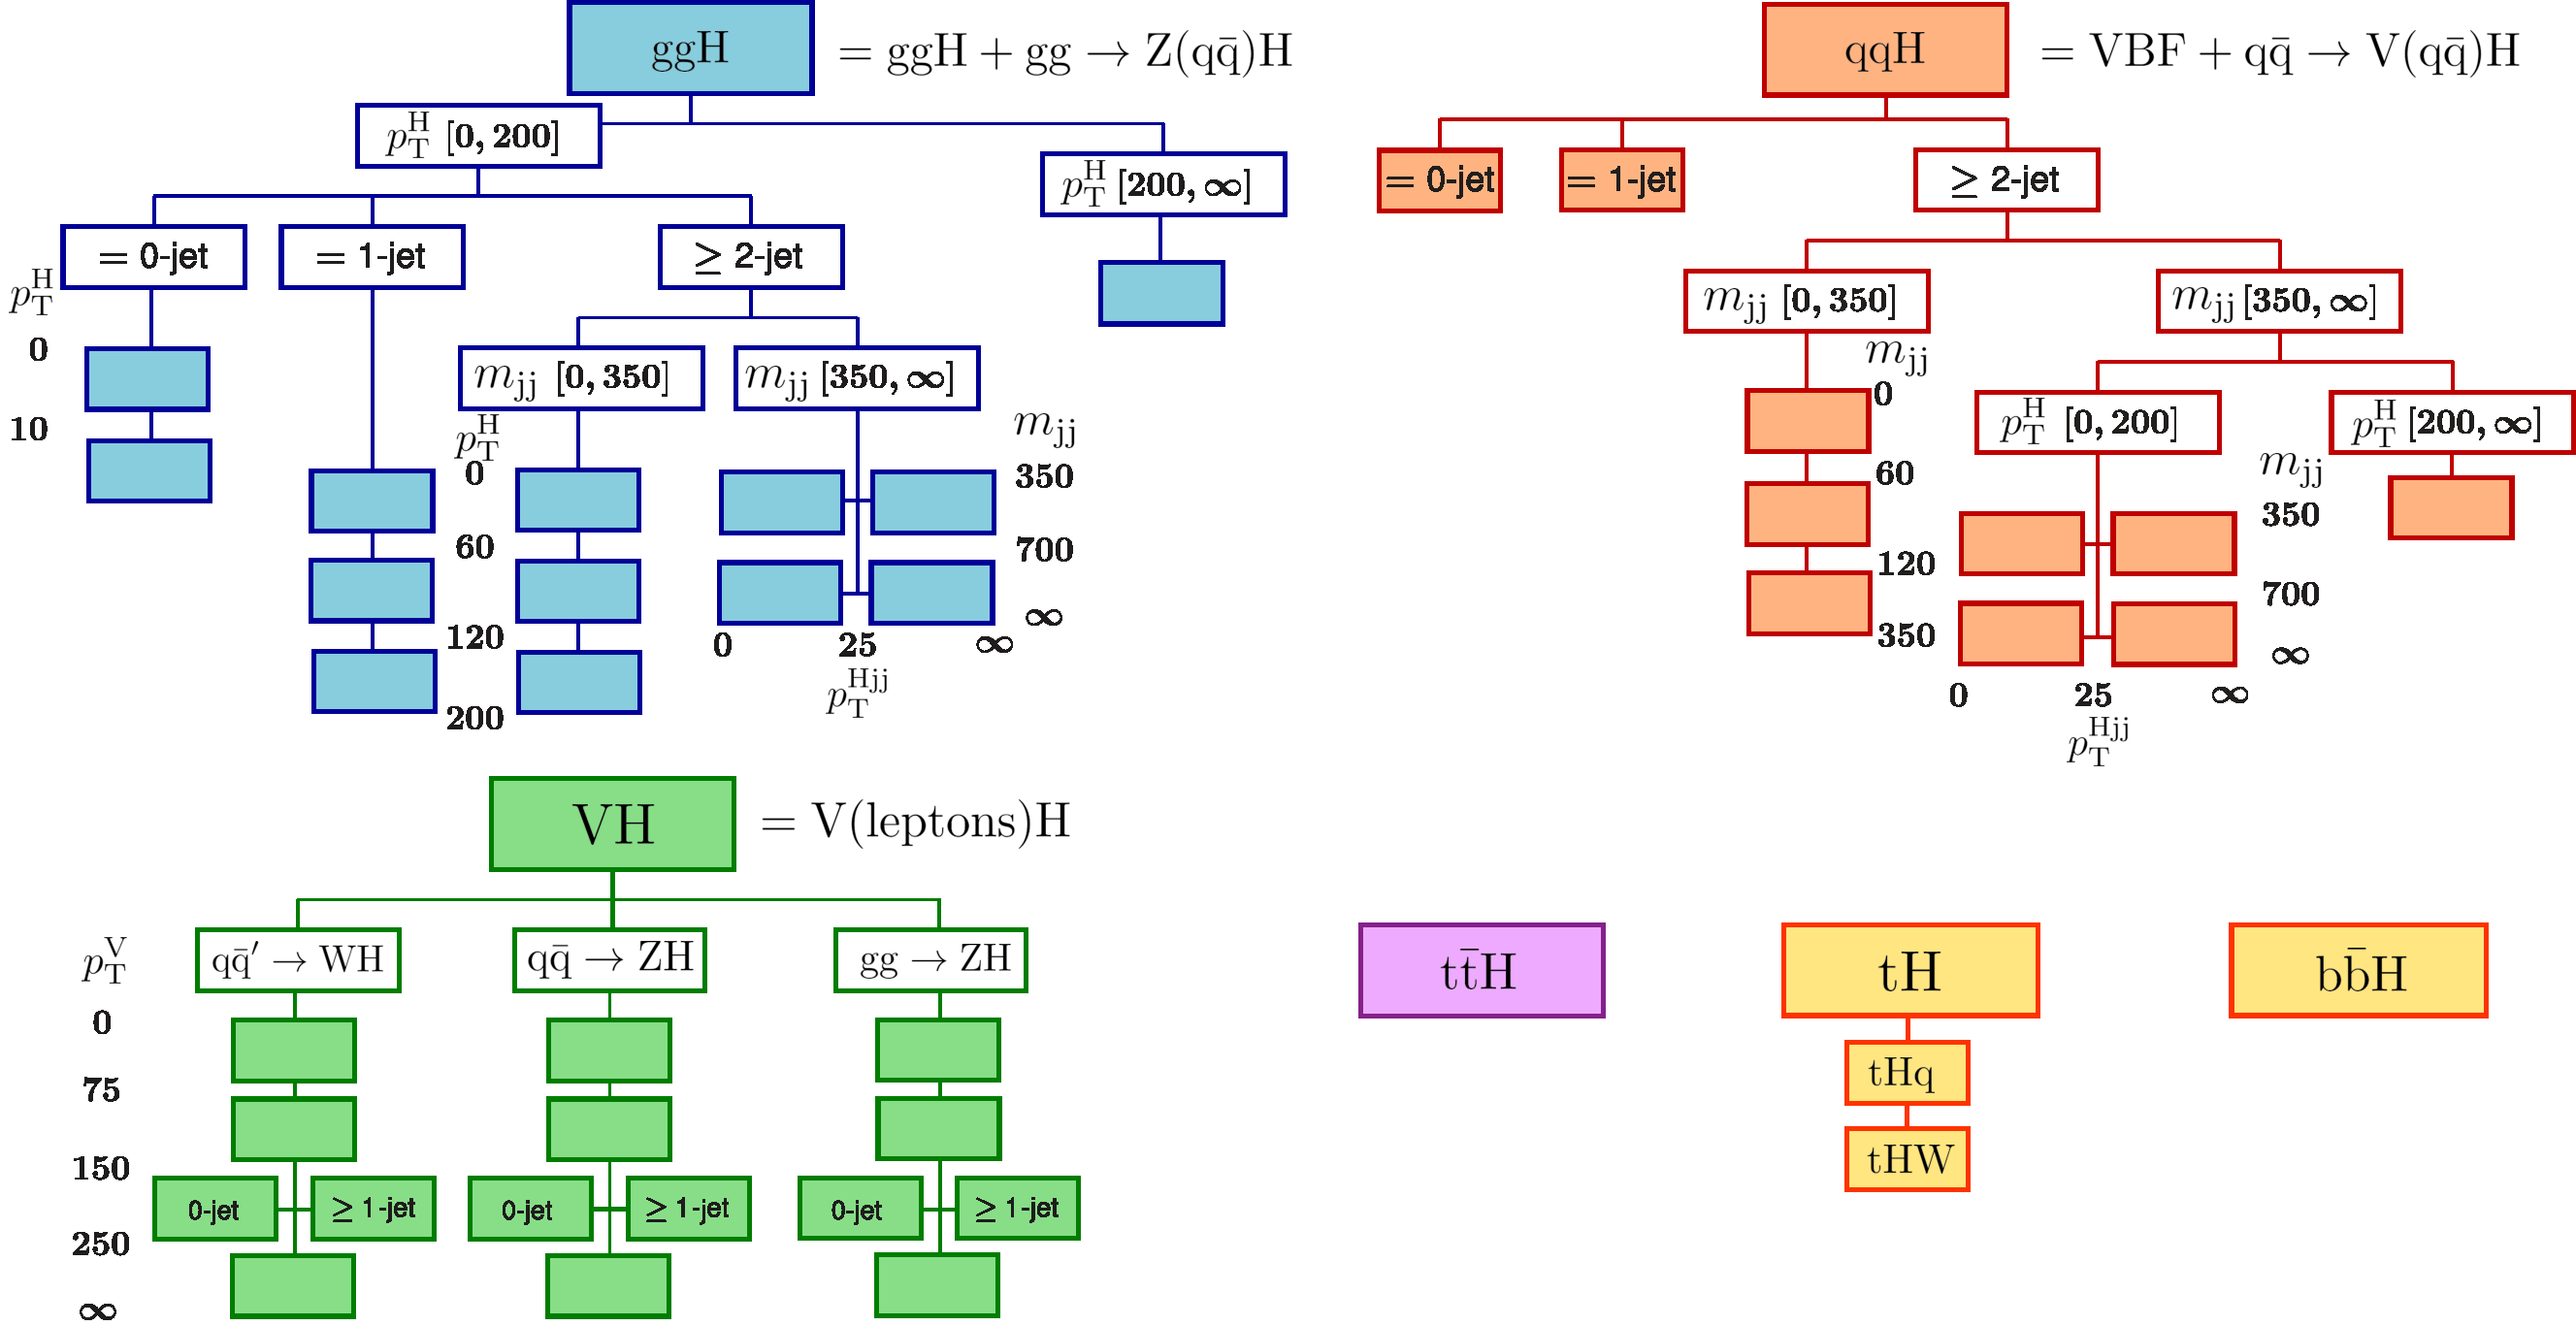
\includegraphics[width=1\linewidth]{Figures/app_merging_schemes/stage1p1.pdf}
  \caption[Schematic of the STXS stage 1.1 binning scheme]
  {
    Add caption
  }
  \label{fig:stxs_schematic_stage1p1}
\end{figure}

\FloatBarrier
\section{Stage 1.2}
\begin{figure}[htb!]
  \centering
  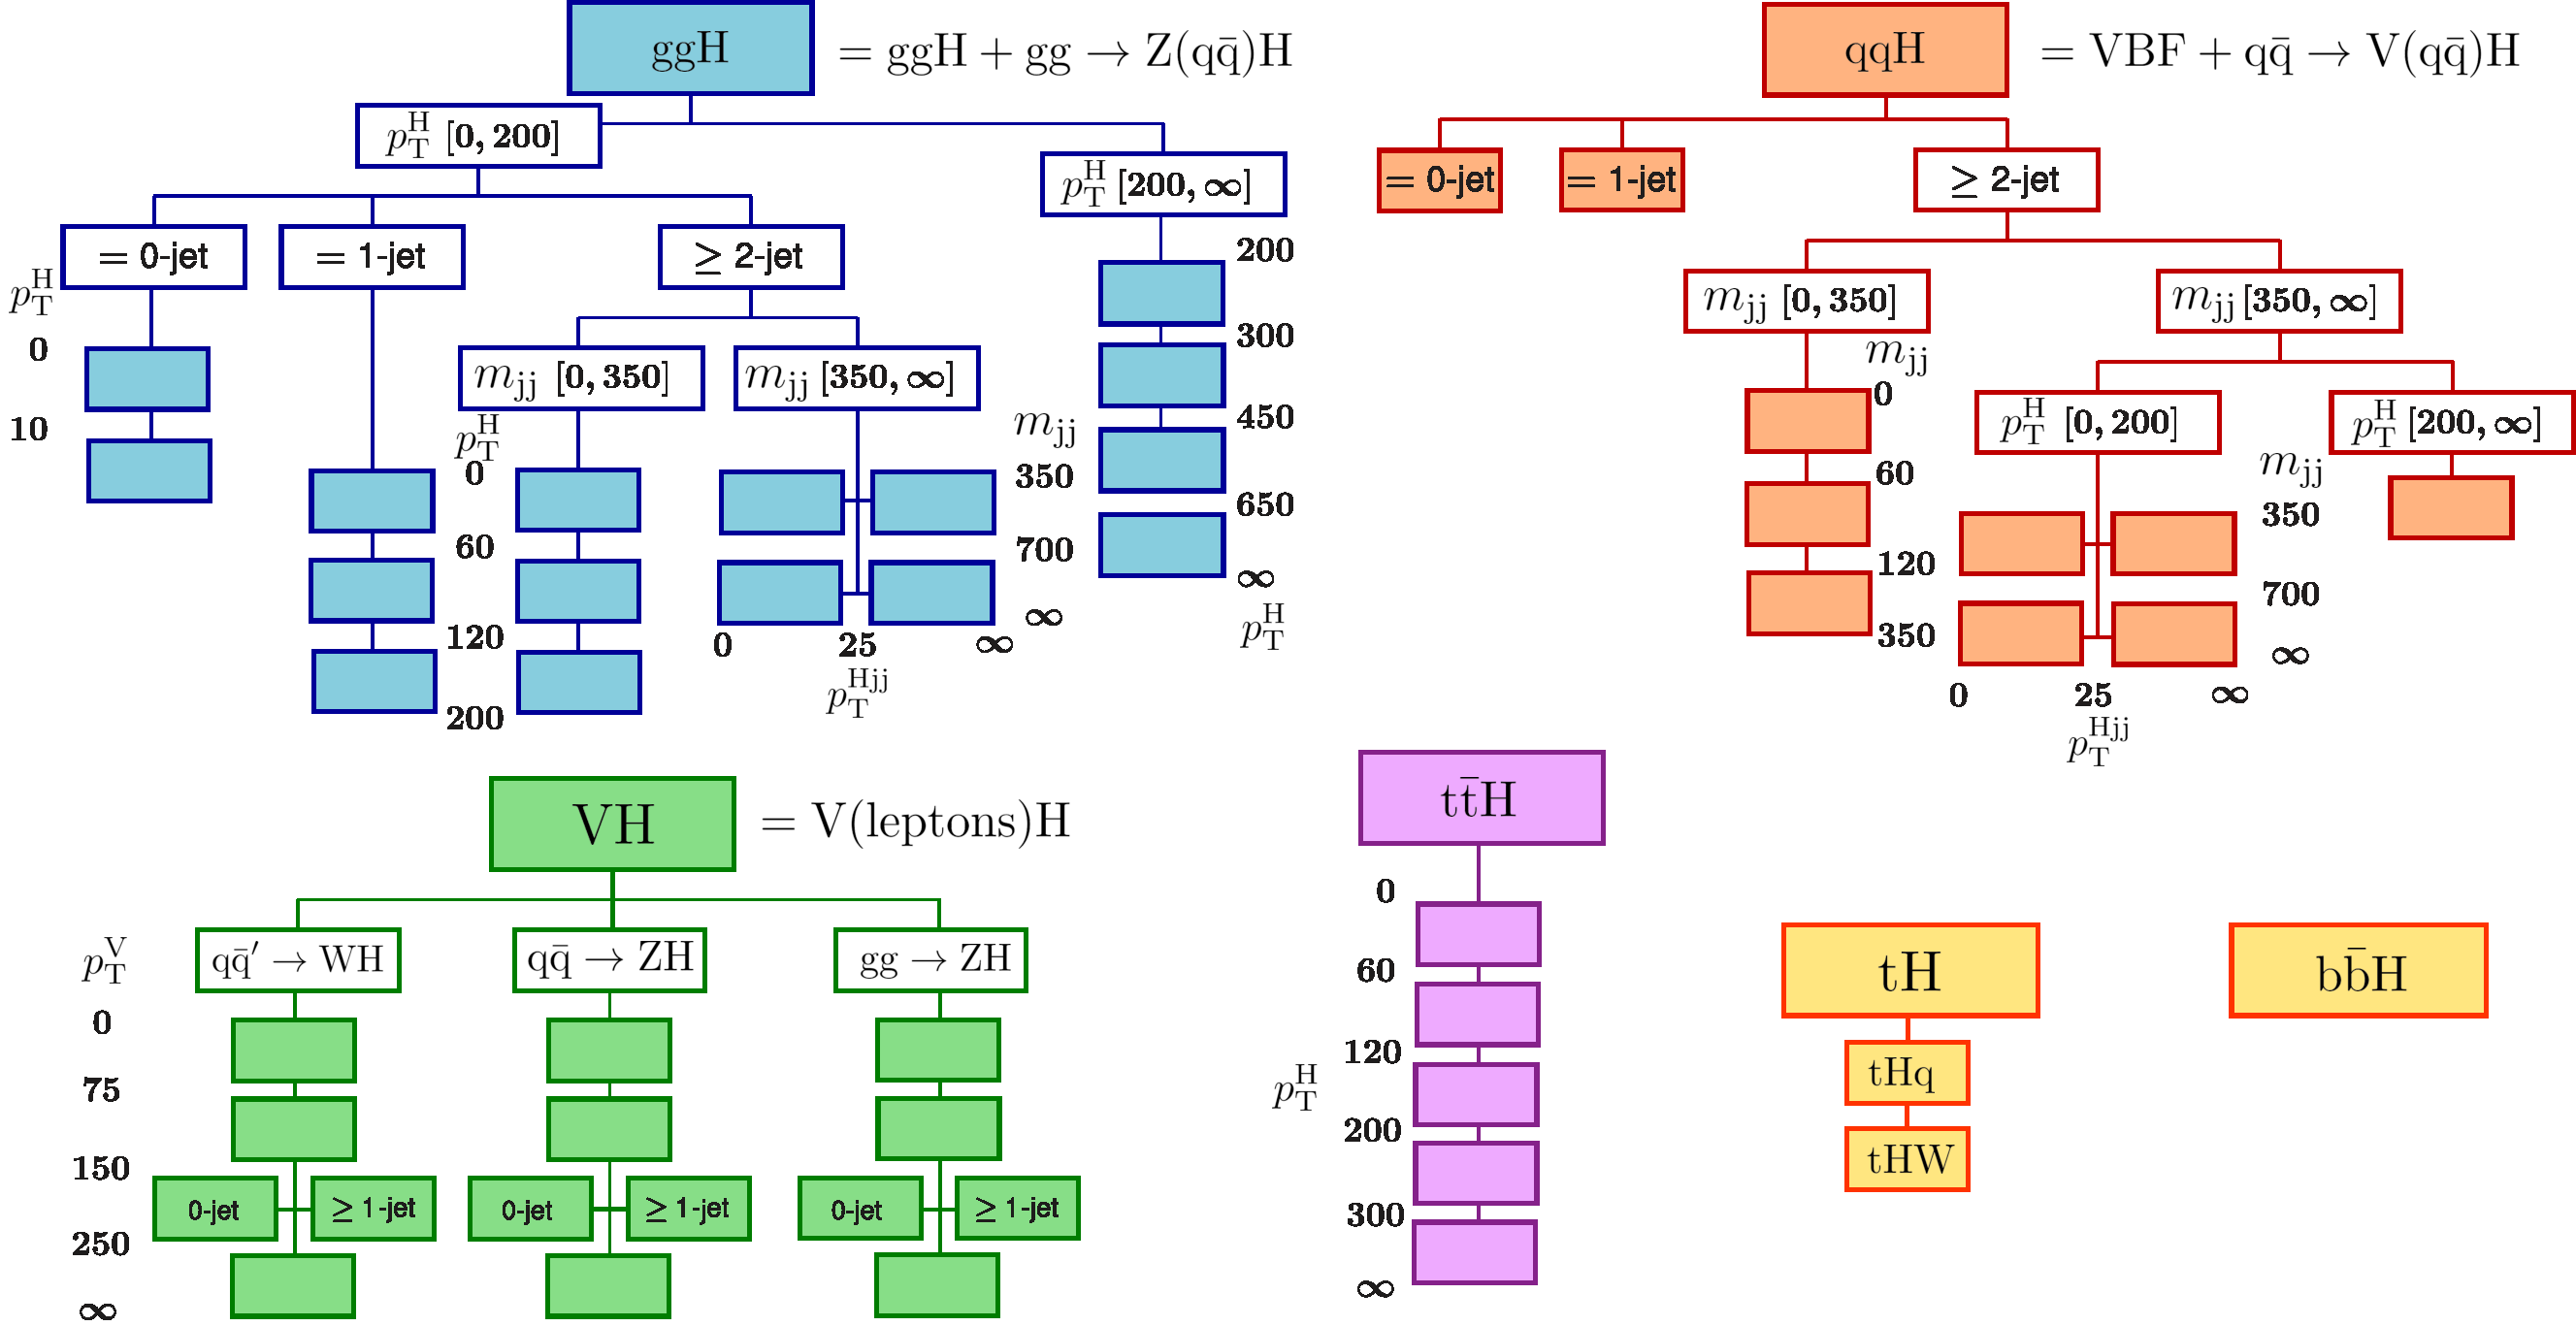
\includegraphics[width=1\linewidth]{Figures/app_merging_schemes/stage1p2.pdf}
  \caption[Schematic of the STXS stage 1.2 binning scheme]
  {
    Add caption
  }
  \label{fig:stxs_schematic_stage1p2}
\end{figure}
